\chapter{Improved Modeling}

Modeling complex human-machine systems is a very difficult and time-consuming task.  This is evidenced by the shear number of modeling approaches to systems involving humans (ACT-R, Soar, DIARC, Brahms, EOFM), the panel \"Modeling Hurts\" at the upcoming AAAI workshop on Formal Methods in Human-Machine Systems, and our own experiences in generating the UE-WiSAR models.  By constructing the MAF Modeling Interface as a set of Java interfaces and abstract classes it meant that the framework was almost entirely extensible in any direction.  We found this very refreshing during the first few development iterations of the framework and model.  We quickly began creating Actors, sub-Actors, Events, and more.  Each transition used an anonymous method containing logic for enabling the transition.  Eventually as our model grew in size and complexity the freedom of the Java language became a dual edged sword.  Our model was full of implicit declarations, inconsistencies, duplicated code, and anonymous methods which are difficult to debug.  It became extremely difficult to maintain the model let alone add to it.  More importantly, it became almost impossible to know if the models were valid and error-free.  This also made it difficult to rely on the metrics we were gathering as each Actor and Transition could implement metric reporting differently.  This chapter discusses an approach to creating MAF models which reduce these problems.

\section{Our Approach}

One approach for improving modeling efficiency is to create GUIs which help the user visualize the model in a way which allows them to more easily understand and make changes to the model.  An example of this is the Brahms Composer~\ref{seah2005multi} which allows the user to create models on the GUI and to visualize the model in different ways.  Another simpler approach is to use a language structure which is human readable and facilitates the creation of an accurate mental model.  An example of this is EOFM~\ref{bolton2009enhanced} which uses an XML structure which can be visualized as a tree graph.  The last approach we will mention is the use of design patterns and object oriented principles to build models which do not exhibit these problems.  The downside to this approach is it then requires the modelers be an expert at Java programming to build error-free models.

While others have successfully taken the third approach, for this thesis we chose to take an approach similar to that of EOFM by constructing an XML structure which represents a labeled state transition system.  Unlike EOFM the XML structure is not the main modeling language.  The XML structure represents a subset of the MAF language which is represented by the underlying Java objects which implement the MAF Modeling Interface.  We chose this approach for several reasons:  XML is commonly used for modeling and other similar tasks, it is simple to work with in Java, it is human readable, and it is structured.  This gave us confidence that we would be able to represent any model in XML and that it could then be converted back into Java.  We also chose this approach because the XML is semantically constrained to the structure we define.  The modeler needs only a basic understanding of XML structures to implement a model.  Another reason for this approach was that it matches the MAF design.  MAF represents a top down approach to abstraction, meaning that the top level Actors, States, Transitions, and Channels are very abstract.  Each subsequent layer removes a portion of that abstraction.  The XML extension adds constraints, to the top level Modeling Interface, which are designed to remove unwanted abstraction from the modeling language itself.  In this case that abstraction was in the form of unnecessary modeling capabilities.

\section{XML Structure}

We defined the following XML structure to represent the labeled state transition system which is given sent to the Simulator.  

The root node is the \em{team} element which consists of the \em{name} attribute and three child elements: \em{channels}, \em{actors}, and \em{events}.

\begin{spacing}{.5}
\lstinputlisting[language=XML]{xml_team.xml}
\end{spacing}

\subsection{Channels}

The \em{channels} element represents the DiTG and is comprised of any number of \em{channel} elements.  Each \em{channel} element represents a single uni-directional communication channel between a source Actor and a target Actor with attributes for the name, type, source, target, and optional dataType.  This is the only location in the XML that defines channels.  Every other \em{channel} element references one of these channels by using the channel name as its value.

\begin{spacing}{.5}
\lstinputlisting[language=XML]{xml_channels.xml}
\end{spacing}

\subsection{Actors}

The \em{actors} element represents the DiRGs contained in the model and is comprised of one or more \em{actor} elements.  Each \em{actor} has a name attribute, which must be unique, and a showMetrics attribute and is made up of several child elements.  The \em{inputchannels} and \em{outputchannels} elements are placed here to validate the DiTG.  The \em{actor} may have 0 or more \em{memory} elements which represent declarative memory used internally as part of the labeled state transitions.  The \em{actor} contains a list of 1 or more \em{state} elements inside of the \em{states} element.  Additionally the \em{actor} element must contain a single \em{startState} element with a value that matches the name attribute of one of the \em{states} child elements.

\begin{spacing}{.5}
\lstinputlisting[language=XML]{xml_actors.xml}
\end{spacing}


\subsection{State and Transitions}



\section{XML Model Parser}

\subsection{Attaching to the Simulator}

The actual XMLModelParser class parses the XML which generates the generic XML team, actor, and transition objects.  Each of these generic XML classes lies separate from the core simulation code interacting through interfaces or by extending abstract classes.  This means that the addition of the XML parser does not prevent the use of custom Actors or Transition classes, use of a different model parser, or extension of our existing XML parser.  In fact our XML parser is meant to be extended to handle a more robust set of models.   As we developed a model using this XMLModelParser we had several occasions to extend its capabilities which we discuss later.  Unsurprisingly it was not difficult to extend the XML to accommodate the changes, often requiring less than 100 lines of code (not including changes to the model XML).

\subsection{Validation}

The use of an XMLModelParser also allowed us to add model validation.  Initial attempts at modeling WiSAR have shown us that model validation time increases dramatically as model complexity increases.  By restricting the model to XML, which is parsed into Java classes, we are able to catch many of the basic modeling errors such as typos, an incomplete DiTG, invalid transitions, and more.  The parser tells the modeler exactly where and what the problem was helping the modeler fix the problem.  While this does not prevent all modeling errors the time to model was drastically reduced.  In addition to the model parsing validation we added several layers of debugging output to help catch those errors not caught by the model parser.


\section{Channel Layers}

While constructing the UAS integrated into NAS model we noticed that a lot of state information was being passed simultaneously across the different channels.  The modeling framework only allowed a single object to be sent across a channel at a time.  While this had the potential to send as much data as needed across the channel we had no way of determining how much data was going across the channel.  With the creation of the XML model parser we limited channel objects to Strings, Integers, and Booleans.  This left us with very limited options for sending lots of data, such as a list of GUI alerts, over a channel.  

On examining this problem in detail we decided that our channels were fundamentally flawed.  In earlier development cycles we had attempted to quantify the data being passed over a channel as we felt it may be important aspect of the workload.  Arriving at this problem again but from a different perspective we decided to add channel layers. See figure~\ref{fig:layers}.  Each channel can have any number of layers.  For example, a visual channel from one person to another has two channels, one which analyzes the face and another which analyzes the body.  Their may be more accurate channel layering for this scenario but these layers satisfy this example.  When communication occurs on this visual channel the recipient can examine as many layers as are needed for the given state.  If the person is in a distracted state then maybe they are not looking at the face layer which may in turn reduce the probability of comprehending the corresponding audio channel.   Another good example where this is useful is in GUIs.  Each item that a GUI represents to the user can be represented as a different layer.  The more layers a GUI presents to a user the more complex it becomes which potentially makes it more difficult for a person to analyze.

As part of the metric analysis we can measure how many layers are being output and read on a particular channel and incorporate this into the workload measurements.  We believe that this concept of channel layers creates a more natural flow of information across the DiTG and it does so in a measurable fashion.  We also believe that these types of measurements will be more effective in improving human machine interfaces because it allows the specific outputs of those interfaces to be directly modeled in a way which directly affects the human workload measurements. 

\begin{figure}[h]
\begin{center}
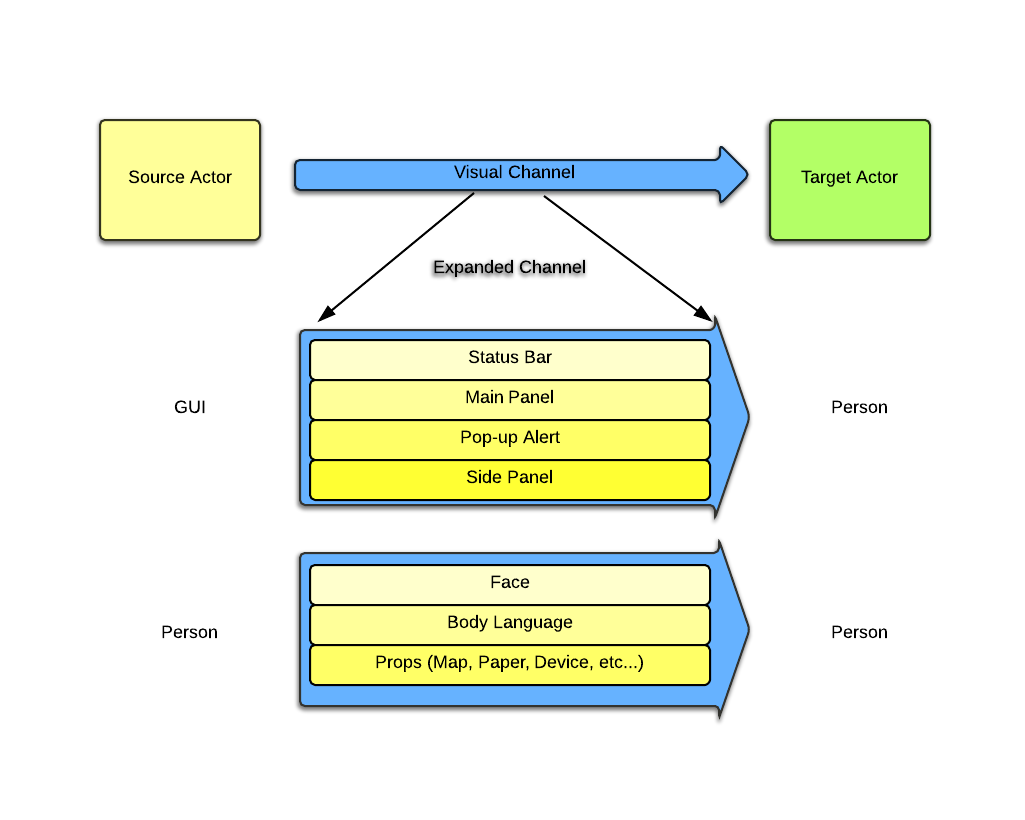
\includegraphics[width=5in]{layers.png}
\caption{Communication Channel Layers}
\label{fig:layers}
\end{center}
\end{figure}
